\section{Einleitung}
Diese Arbeit entstand im Rahmen des Moduls Projekt KI des Verbundstudiengangs Angewandte Informatik an der Fachhochschule Südwestfalen Standort Iserlohn. Sie beschäftigt sich mit der Erstellung eines Bilddatensatzes für die Objekterkennung mit echten und synthetischen Bildern. Nachfolgend wird die Vorgehensweise bei der Erstellung des Datensatzes beschrieben. Dabei wird zuerst auf die Auswahl der Modelle und die Testumgebung für die Auswahl eines Modells eingegangen. Anschließend wird die Erstellung des Datensatzes beschrieben. Dabei wird zuerst auf die Auswahl der echten Bilder und anschließend auf die Erstellung der synthetischen Bilder eingegangen, bevor dann die Annotation der Bilder beschrieben wird. Zum Schluss werden die Ergebnisse des Projekts zusammengefasst.

\subsection{Projekthintergrund}
Dieses Projekt soll als Vorarbeit für die nachfolgende Bachelorarbeit dienen. In dieser soll ein KI-Modell zur Objekterkennung um eine weitere Klasse erweitert werden. Als Grundlage soll der COCO Datensatz verwendet werden \cite{coco2015}. Dabei soll untersucht werden wie gut die Erkennung anhand von echten Bildern und synthetischen (mit einem KI-Modell generierte Bilder) ist.

\subsection{Projektbeschreibung und Ziele}
Ziel dieses Projektes ist es einen Datensatz aus KI generierten (synthetischen) und echten Bildern zu erstellen und diese mit Annotationen zu versehen. Der erstellte Datensatz soll für den Vergleich der Leistung von Objekterkennungsmodellen verwendet werden. Verglichen werden soll die Erkennungsleistung von Modellen zur Objekterkennung an einer neuen Kategorie von Objekten anhand von echten, synthetischen und gemischten Bildern des, in diesem Projekt erstellten, Datensatzes. Als Basis werden Modelle verwendet die auf dem COCO Datensatz \cite{coco2015} trainiert wurden. Dieser umfasst 80 Objektkategorien. Eine Kategorie die darin nicht enthalten ist, sind Musikinstrumente. Aufgrund des zeitlichen Rahmens des Projektes wird die Kategorie dabei auf ein Instrument beschränkt. Da für den COCO Datensatz kein entsprechender Datensatz existiert soll dieser in diesem Projekt erstellt werden.

Der Fokus in diesem Projekt liegt dabei hauptsächlich auf der Erstellung des synthetischen Teils des Datensatzes. Für die Erstellung dieses Teils wird ein lokales (FH Cluster oder lokaler Computer) Text-zu-Bild Modell verwendet, welches die Bilder generieren soll. Zuerst wird nach aktuellen Modellen für die Bildgenerierung recherchiert. Danach werden zwei bis drei der Modelle miteinander verglichen, indem, mit der gleichen Texteingabe, einige Bilder erstellt und verglichen werden. Das beste Modell wird dann weiter verwendet. Als Quelle für Modelle kann zum Beispiel Hugging Face \cite{huggingface2025} dienen. Die zur Bildgenerierung verwendete Umgebung, das Modell und die Texteingabe werden dabei erläutert. Anschlie{\ss}end werden die Bilder mit einer Annotationssoftware aufbereitet. Für die Aufbereitung der Bilder wäre der Einsatz von CVAT \cite{cvat2025} oder Label Studio \cite{labelimg2025} möglich. Beide Programme sind kostenlos und lokal einsetzbar. Hierbei wird erläutert wie die Software bei der Annotation unterstützt und worauf zu achten ist, um einen hochwertigen Datensatz zu erstellen.

\subsection{Zeitplanung}
Das Gantt-Diagramm \ref{gantt} zeigt die Zeitplanung für dieses Projekt. Die Planung enthält die verschiedenen Phasen und Meilensteine. Bei der Planung der Dauer der einzelnen Phasen wurde berücksichtigt, dass auch weitere Projekte anderer Module durchgeführt werden. Die Phasen wurden entsprechend länger angesetzt.
	
	Die erste Phase Recherche und Vergleich von Modellen umfasst die Recherche nach aktuellen Bildgenerierungsmodellen und deren Evaluation anhand von testweise erstellten Bildern mit den Modellen. In der zweiten Phase Aufbau Umgebung Bildgenerierung wird das zuvor ausgewählte Modell und entsprechende Infrastruktur für die Erstellung von einer gro{\ss}en Anzahl an Bildern erstellt. An dieser Stelle ist der Meilenstein Ende Vorbereitung erreicht und die Erstellung der Bilder kann beginnen. Für die Phase Bildgenerierung und Aufbereitung ist ein Zeitraum von sechs Wochen vorgesehen. In dieser Zeit sollen so viele Bilder wie möglich erstellt und gelabelt werden. Es wird dabei eine Anzahl von 100 Bildern anvisiert. Nach dieser Phase ist der zweite Meilenstein erreicht und es wird in der letzten Phase mit der Dokumentation begonnen.
	
	\noindent % Entfernt Einrückung
	\resizebox{\textwidth}{!}{ % Verkleinert das Diagramm
		\begin{ganttchart}[
			hgrid,
			vgrid,
			x unit=0.7cm, % Verkleinert die Balkenbreite
			y unit title=0.7cm,
			y unit chart=0.6cm,
			time slot format=simple
			]{1}{16}
			\gantttitle{Projektzeitraum (16 Wochen)}{16} \\
			\gantttitlelist{1,...,16}{1} \\
			\ganttbar{Recherche und Vergleich von Modellen}{1}{3} \\
			\ganttbar{Aufbau Umgebung Bildgenerierung}{4}{4} \\
			\ganttmilestone{Ende Vorbereitung}{4} \\
			\ganttbar{Bildgenerierung, Sammlung und Aufbereitung}{5}{10} \\
			\ganttmilestone{Ende praktische Durchführung}{10} \\
			\ganttbar{Dokumentation}{11}{16}
            \label{gantt}
		\end{ganttchart}
	}


\section{Durchführung}
Den Start des Projekts bildet das Kickoff-Meeting mit dem Projektbetreuer und dem Projektdurchführenden am 29.03.2025.
In diesem Meeting wurde das Projekt vorgestellt und die Ziele sowie der Zeitplan besprochen. Anschließend wurde mit der Abgabe des Projektantrags das Projekt offiziell angemeldet.
\subsection{Recherche und Vergleich von Modellen}
Das Projekt beginnt mit der Recherche nach aktuellen KI-Modellen, die für die Generierung von Bildern geeignet sind. Dafür wurde zuerst nach entsprechend Benchmarks für die Vergleich von Modellen gesucht. Ein solcher Benchmark hätte es ermöglicht, die Modelle direkt miteinander zu vergleichen und die besten Modelle für das Projekt auszuwählen. Leider gibt es keinen allgemeingültigen Benchmark, der für alle Modelle geeignet ist. Daher wurde beschlossen, die vier obersten Modelle auf der Hugging Face Website unter der Kategorie Text-To-Image, nach der Sortierung Trending, zu vergleichen. Dabei wurden verschiedene Versionen des gleichen Modells nicht berücksichtigt und jeweils das größte Modell ausgewählt. Fine-Tunings von Modellen wurden auch aus der Auswahl ausgeschlossen um einen möglichst repräsentativen Vergleich von verschiedenen Architekturen zu erhalten. Daraus entstand am 17.04.2025 die folgende Liste von Modellen, die für den Vergleich verwendet werden:
\begin{itemize}
    \item HiDream-ai/HiDream-I1-Full
    \item black-forest-labs/FLUX.1-dev
    \item stabilityai/stable-diffusion-3.5-large
    \item stabilityai/stable-diffusion-xl-base-1.0
\end{itemize}
Diese Liste stellt die Modelle in der Reihenfolge dar, in der sie nach der Trending Sortierung angezeigt wurden.
\subsection{Kurzvorstellung der Modelle}
% Kurzvorstellung der Modelle
% Hier Potenzial zum erweitern durch erklären der Techniken
HiDream-I1-Full ist das neueste der vier Modelle es wurde Anfang April 2025 von Vivago AI als Open-Source Modell veröffentlicht. Es ist in den Varianten HiDream-I1-Full, HiDream-I1-Dev, HiDream-I1-Fast als Text-zu-Bild oder als HiDream-E1 für die Bearbeitung von Bildern verfügbar. Nach eigenen Angaben im entsprechenden Paper \cite[Abstract]{cai2025hidreami1highefficientimagegenerative} wurden neueste Fortschritte bei der Verbesserung der Qualität von Bildern durch eine Steigerung der Rechenkomplexität erzielt. Dies führe zu besseren Ergebnissen aber auch zu längeren Inferenzzeiten. Um diesem Problem entgegenzuwirken, wurde das HiDream-I Modell entwickelt um hochwertige Ergebnisse in kurzer Zeit zu liefern.
Um dies zu erreichen wurde eine neue Architektur entwickelt, der \emph{Sparse Diffusion Transformer}. Das Modell verwendet zunächst drei Encoder um die Texteingabe zu verarbeiten. Anschließend folgt ein \emph{Dual-stream Diffusion Transformer} (DiT) Block der die Texteingabe und die Bilddaten getrennt verarbeitet. Diese beiden Streams werden dann in einem \emph{Single-stream} DiT Block zusammengeführt. 
Beide Blöcke verwenden ein \emph{sparse Mixture-of-Experts} (MoE) Konzept um gezielt Teile des Bildes zu verarbeiten. Die Experts werden dabei von einen \emph{dense feed-forward network} (FNN), welches als Router fungiert, gespeist. Durch die gezielte, spärliche, Aktivierung der Experts lässt sich die benötigte Rechenleistung reduzieren.
Das vollständige Modell besitzt 17 Milliarden Parameter und ist damit das größte Modell in dieser Auswahl \cite[S.~7-9]{cai2025hidreami1highefficientimagegenerative}.

Das Flux.1 Modell wurde im August 2024 von Black Forest Labs (BFL), eines in Freiburg im Breisgau gegründeten Start-Ups, veröffentlicht. Es ist in den drei Varianten FLUX.1-pro, FLUX.1-dev und FLUX.1-schnell verfügbar, wobei das FLUX.1-pro Modell nicht frei verfügbar ist. 
Das Modell basiert nach eigenen Angaben von BFL auf ihrer Webseite aus ``einer hybriden Architektur aus multimodal und parallel diffusion Transformer Blöcken die auf 12 Milliarden Parameter skaliert wurden. Die Architektur wird durch flow Matching weiter verbessert. Die Performance und Hardwareeffizienz wird durch den Einsatz von rotary positional embeddings und parallel attention layers optimiert'' \cite{bfl-flux-announcement}.

Das Stable Diffusion 3.5 stammt von Stability AI und wurde im Oktober 2024 veröffentlicht. Es ist in den Varianten Large, Large Turbo und Medium verfügbar. Diese dürfen für die Forschung, für nicht-kommerzielle und kommerzielle bis zu einem Jahresumsatz von einer Million US Dollar frei verwendet werden.
Die in diesem Projekt verwendete Large Variante hat 8.1 Milliarden Parameter. Dieses Modell setzt auf eine multimodal Diffusion Transformer Architektur (MMDiT). Dies erlaubt es entgegen anderen Architekturen, wie zum Beispiel der einfachen Diffusion Transformer Architektur, dass eine Zwei-Wege Kommunikation zwischen den Text und Bild Daten stattfindet. Dies erlaubt eine bessere Text-zu-Bild Generierung. Trainiert wurde das Modell auf dem ImageNet und CC12M Datensatz und wurde gegen den COCO-2014 Validierungssatz getestet \cite[S.~4-5]{esser2024scalingrectifiedflowtransformers}.

Das Stable Diffusion XL (SDXL) Modell stammt auch von Stability AI und wurde im Juli 2023 veröffentlicht. Es basiert auf Stable Diffusion 2.1 ist aber mit 3,5 Milliarden Parameter eine dreimal größer als sein Vorgänger. Dies liegt an einem größeren attention block und einem größeren cross-attention context durch einen zweiten Text Encoder. Genau wie der Vorgänger Stable Diffusion 2.1 basiert es auf einem Latent Diffusion Model mit einem UNET zur Reduzierung des Rauschens in den Bildern \cite[Abstract]{podell2023sdxlimprovinglatentdiffusion}.
Die Besonderheit bei diesem Modell besteht darin, dass es ich hierbei um ein Assemble of Experts Modell handelt. Dabei handelt es sich um die zwei Modelle Stable Diffusion XL Base und Stable Diffusion XL Refiner, die zusammen verwendet werden. Das Base Modell generiert dabei ein erstes Bild, welches dann vom Refiner Modell, welches auf die Erstellung von Details angepasst wurde, weiter verfeinert wird. Dadurch soll eine höhere Qualität der Bilder erreicht werden \cite[S.~2]{podell2023sdxlimprovinglatentdiffusion}.


\subsection{Erstellung der Testumgebung}
Für den Vergleich der Modelle wurde eine Testumgebung in einem Juyper Notebook erstellt. Der Code ist in der beiliegenden Datei \texttt{evaluation-of-image-model.ipynb} zu finden. 
Für die Ausführung der Modelle mit der Hugging Face diffusers-Bibliothek \cite{von-platen-etal-2022-diffusers} muss momentan (Stand 26.05.2025) die Bibliothek aus dem diffusers GitHub Repository installiert werden, da die aktuellste veröffentlichte Version der Bibliothek (v0.33.1 vom 10.04.2025) nicht die Pipeline für das HiDream Modell enthält. Zudem wird ein Hugging Face Token benötigt, um auf die Tokenizer und Encoder, des von HiDream benötigten, \texttt{meta-llama/Meta-Llama-3.1-8B-Instruct} Modells zugreifen zu können.
Für eine einfache Ausführung der Modelle wurde eine Funktion erstellt, die eine Modell Pipeline und einige Parameter entgegennimmt und dann Bilder generiert und diese in einem Verzeichnis abspeichert. Die Funktion generiert für jede Texteingabe drei Bilder, wobei der \emph{guidance\_scale} um den, vom Modell empfohlenen Wert, plus eins und minus eins variiert wird. Die Anzahl der Schritte wird der Funktion beim Aufruf mitgegeben und entspricht der vom Modell empfohlenen Anzahl.
Die definierte Funktion wird dann nach dem Laden der Modelle über die jeweiligen Pipelines aufgerufen.

Die Tests der Modelle wurden auf dem JuyperHub der Fachhochschule Südwestfalen durchgeführt. Dort werden verschiedene Python-Umgebungen bereitgestellt und bieten Zugriff auf verschiedene GPU Konfigurationen mit Nvidia A100 Grafikkarten mit 80 GB VRAM. Die zuerst verwendete Konfiguration bietet einen geteilten Zugriff auf 4 A100 Grafikkarten. Dies führte zu Problemen bei der Ausführung der Modelle, da nicht ausreichend VRAM für die Modelle, insbesondere für das HiDream Modell, zur Verfügung stand. Daher wurde für das weitere Vorgehen eine Konfiguration mit einer dedizierten A100 Grafikkarte mit 40 GB VRAM gewählt.
Diese Konfiguration bot für einen ausreichenden Zeitraum Zugriff auf ausreichend VRAM für die meisten Modelle. Lediglich das HiDream Modell stieß weiterhin auf Probleme mit dem Speicher. Diese konnten durch die Aktivierung von zwei Flags in der Pipeline behoben werden. Die Flags waren \emph{enable\_model\_cpu\_offload} und \emph{enable\_vae\_tiling}. Das Flag \emph{enable\_model\_cpu\_offload} sorgt dafür, dass das Modell nicht vollständig im VRAM gehalten wird, sondern im RAM und Submodule bei Bedarf in den VRAM geladen werden. Dadurch lässt sich der beötigte GPU-Speicher reduzieren, zum Preis einer längeren Ausführzeit, da die Module zwischen Speichern hin und her geladen werden müssen.
Das Flag \emph{enable\_vae\_tiling} sorgt dafür, dass der VAE (Variational Autoencoder) des Modell das Bild in sich überlappenden Kacheln verarbeitet und diese am Ende wieder zusammensetzt. Dadurch kann der benötigte Speicher für die Verarbeitung für größere Bilder reduziert werden \cite{hf-memory-optimization}.

Als Texteingaben für die Modelle wurden zwei verschiedene Eingaben gewählt. Diese sind:
\begin{itemize}
    \item a hyperrealistic photo of a group of musicians playing various instruments in a band, set in a random location
    \item a hyperrealistic photo of a common living room with a variety of music instrument scattered around the room
\end{itemize}
Diese beiden Texteingaben wurden gewählt um ein möglichst breites Spektrum an Instrumenten und Szenen zu generieren. Das Ziel dabei war es ein Modell auszuwählen, dass mit einer möglichst allgemeinen Texteingabe möglichst viele verschiedene Instrumente in verschiedenen Szenen generieren kann. Mit dem Zusatz \emph{hyperrealistic photo} soll dabei sichergestellt werden, dass die generierten Bilder möglichst realistisch aussehen. 
Mit diesem Testaufbau wurden dann insgesamt 24 Bilder erstellt.

\subsection{Vergleich der Modelle}
Für die Auswahl des Modells wurden verschiedenen Kriterien festgelegt, die für ein Modell welches den Anforderungen des Projekts gerecht werden soll, wichtig sind.

Das erste Kriterium ist die Anzahl der Fehler in den Bild. Für dieses Kriterium wurden die generierten Bilder durch den Autor auf visuelle Fehler untersucht. Als visueller Fehler wird dabei eine Abweichung von einem realen Bild der gleichen Szene definiert. Dies können Artefakte, falsche Anatomie von Personen oder Fehler in der Darstellung der Instrumente sein.\\
Das zweite Kriterium ist die Diversität der dargestellten Instrumente. Da in der nachfolgenden Bachelorarbeit ein Modell für Objekterkennung von Gitarren trainiert werden soll, ist es wichtig, dass das Modell verschiedene Gitarren darstellen kann, aber auch andere, ähnliche, Instrumente wie Geigen, Cellos, oder Banjos. Die Diversität wird dabei als Anzahl unterschiedlicher Instrumente und deren Variationen in den generierten Bildern definiert. Dafür wird die Anzahl der verschiedenen Instrumente in den generierten Bildern gezählt. Eine Variation eines Instruments wird mit einem halben Punkt bewertet und ein neues Instrument mit einem Punkt. Die Punkte werden dann addiert und ergeben die Diversität der Instrumente in den generierten Bildern.\\
Das dritte Kriterium ist die Diversität der Szene. Diese wird ähnlich wie die Diversität der Instrumente bewertet. Pro Modell werden Bilder mit zwei Eingaben generiert. Die Modelle verwenden dabei die empfohlenen Parameter, wobei pro Eingabe drei Bilder erstellt werden. Pro Bild variiert der \emph{guidance\_scale} um den, vom Modell, empfohlenen Wert plus zwei und minus zwei. Jede Szene wird dabei mit einem Punkt bewertet. Eine Variation einer bereits vorhandenen Szene wird mit einem halben Punkt bewertet.\\
Die Gesamtwertung pro Bild wird dann aus der Summe der Punkte der Diversitätskriterien abzüglich der Anzahl der Fehler in den Bildern gebildet. Für die Modellwertung werden dann die Einzelwertungen addiert und durch die Anzahl der Bilder geteilt. Das Modell mit der höchsten Gesamtwertung wird dann als das beste Modell ausgewählt.\\
In Tabelle \ref{modelevaluationresults} sind die Ergebnisse der Bewertung der Modelle dargestellt. Die untersuchten Bilder mit den markierten Fehlern und Instrumenten sind im Projektordner \texttt{eval\_files\_marked} zu finden. Eine Auswahl von Bildern ist in der Abbildung \ref{fig:marked_images} zu sehen.

\begin{figure}
    \begin{minipage}{0.24\textwidth}
        \centering
        \includegraphics[width=\textwidth]{bilder/HiDream-I1-Full_prompt-0_guidance-7.0_steps-50.png}
    \end{minipage}
    \begin{minipage}{0.24\textwidth}
        \centering
        \includegraphics[width=\textwidth]{bilder/FLUX-1-dev_prompt-0_guidance-3.5_steps-50.png}
    \end{minipage}
    \begin{minipage}{0.24\textwidth}
        \centering
        \includegraphics[width=\textwidth]{bilder/sd35_prompt-0_guidance-5.5_steps-28.png}
    \end{minipage}
    \begin{minipage}{0.24\textwidth}
        \centering
        \includegraphics[width=\textwidth]{bilder/sdxlrefiner_prompt-0_guidance-9.5_steps-40.png}
    \end{minipage}
    \caption{Eine Auswahl an markierten Bildern für die Bewertung der Modelle. Von links nach rechts: HiDream-I1-Full, FLUX.1-dev, Stable Diffusin 3.5 Large, Stable Diffusion XL Refiner.}
    \label{fig:marked_images}
\end{figure}

\begin{table}[]
    \centering
    \resizebox{\textwidth}{!}{
        \begin{tabular}{llllll}
        \toprule
        Dateiname & \makecell{Anzahl\\Fehler} & \makecell{Diversität\\Instrumente} & \makecell{Diversität\\Szene} & Wertung \\
        \midrule
        HiDream-I1-Full\_prompt-0\_guidance-3.0\_steps-50.png & 7 & 3,5 & 1   & -2,5 \\ \addlinespace
        HiDream-I1-Full\_prompt-0\_guidance-5.0\_steps-50.png & 9 & 1,5 & 0,5 & -7 \\ \addlinespace
        HiDream-I1-Full\_prompt-0\_guidance-7.0\_steps-50.png & 8 & 4   & 0,5 & -3,5 \\ \addlinespace
        HiDream-I1-Full\_prompt-1\_guidance-3.0\_steps-50.png & 5 & 2   & 1   & -2 \\ \addlinespace
        HiDream-I1-Full\_prompt-1\_guidance-5.0\_steps-50.png & 5 & 1   & 0,5 & -3,5 \\ \addlinespace
        HiDream-I1-Full\_prompt-1\_guidance-7.0\_steps-50.png & 3 & 2,5 & 0,5 & 0 \\ \addlinespace
        FLUX-1-dev\_prompt-0\_guidance-1.5\_steps-50.png & 2 & 2,5 & 1 & 1,5 \\ \addlinespace
        FLUX-1-dev\_prompt-0\_guidance-3.5\_steps-50.png & 4 & 3   & 1 & 0 \\ \addlinespace
        FLUX-1-dev\_prompt-0\_guidance-5.5\_steps-50.png & 3 & 4   & 1 & 2 \\ \addlinespace
        FLUX-1-dev\_prompt-1\_guidance-1.5\_steps-50.png & 2 & 1   & 1 & 0 \\ \addlinespace
        FLUX-1-dev\_prompt-1\_guidance-3.5\_steps-50.png & 1 & 3,5 & 1 & 3,5 \\ \addlinespace
        FLUX-1-dev\_prompt-1\_guidance-5.5\_steps-50.png & 1 & 3,5 & 1 & 3,5 \\ \addlinespace
        sd35\_prompt-0\_guidance-1.5\_steps-28.png & 2 & 1   & 1 & 0 \\ \addlinespace
        sd35\_prompt-0\_guidance-3.5\_steps-28.png & 2 & 2,5 & 1 & 1,5 \\ \addlinespace
        sd35\_prompt-0\_guidance-5.5\_steps-28.png & 4 & 3   & 1 & 0 \\ \addlinespace
        sd35\_prompt-1\_guidance-1.5\_steps-28.png & 5 & 3   & 1 & -1 \\ \addlinespace
        sd35\_prompt-1\_guidance-3.5\_steps-28.png & 4 & 3,5 & 1 & 0,5 \\ \addlinespace
        sd35\_prompt-1\_guidance-5.5\_steps-28.png & 5 & 2,5 & 1 & -1,5 \\ \addlinespace
        sdxlrefiner\_prompt-0\_guidance-5.5\_steps-40.png & 7 & 0 & 1 & -6 \\ \addlinespace
        sdxlrefiner\_prompt-0\_guidance-7.5\_steps-40.png & 7 & 0 & 1 & -6 \\ \addlinespace
        sdxlrefiner\_prompt-0\_guidance-9.5\_steps-40.png & 8 & 0 & 1 & -7 \\ \addlinespace
        sdxlrefiner\_prompt-1\_guidance-5.5\_steps-40.png & 7 & 0 & 1 & -6 \\ \addlinespace
        sdxlrefiner\_prompt-1\_guidance-7.5\_steps-40.png & 8 & 0 & 1 & -7 \\ \addlinespace
        sdxlrefiner\_prompt-1\_guidance-9.5\_steps-40.png & 7 & 1 & 1 & -5 \\ \addlinespace
        \bottomrule
        \end{tabular}
    }
    \caption{Bewertung der Modelle}
    \label{modelevaluationresults}
\end{table}

Anhand der Ergebnisse des Vergleichs der Modelle in Tabelle \ref{modelevaluationresults} sieht man, dass die Bilder des Modells Stable Diffusion XL (SDXL) mit 44 die meisten Fehler aufweisen. Das Modell HiDream-I1-Full hat mit 34 Fehlern die zweitmeisten Fehler. Mit einem Abstand von 12 Fehlern folgt das Modell Stable Diffusion 3.5 Large (SD35) mit 22 Fehlern. Das Modell FLUX.1-dev hat, mit einem Abstand von 9, die wenigsten Fehler mit insgesamt nur 13 Fehlern.
Bei der Diversität der Instrumente fällt besonders auf, dass das Modell SDXL nur einen einzigen Punkt für die Instrumente erhält. Dies liegt an der Tatsache, dass es nur ein einziges erkennbares Instrument in allen Bilern erstellt hat. An vorletzter Stelle befindet sich das HiDream Modell mit einer Punktzahl von 13,5. Knapp davor mit 14 Punkten liegt das SD35 Modell. Mit einem Abstand von 1,5 Punkten bietet das FLUX.1 Modell mit einer Punktzahl von 15,5 die größte Diversität an Instrumenten.
In der letzten Bewertungskategorie, der Diversität der Szenen, haben fast alle Modelle die volle Punktzahl von erhalten, da sie in jedem Bild eine andere Szene erstellt haben. Nur das HiDream Modell erhält mit 4 Punkten eine niedrigere Wertung, da es viermal nur eine Variation einer bereits erstellten Szene enthielt.

Basierend auf den Ergebnissen aus Tabelle \ref{modelevaluationresults} ergeben sich die folgenden Gesamtwertungen für die Modelle:
\begin{itemize}
    \item HiDream-I1-Full: -3
    \item FLUX-1-dev: 1,75
    \item sd35: 0,08
    \item sdxlrefiner: -6,1
\end{itemize}

Das Modell FLUX.1 dev hat die höchste Gesamtwertung und wird daher für die weitere Arbeit verwendet. Das Modell Stable Diffusion 3.5 Large (sd35) hat zwar auch eine positive Gesamtwertung, jedoch ist die Diversität der Instrumente und Szenen geringer als bei dem FLUX-Modell. Die Modelle HiDream-I1-Full und Stable Diffusion XL Refiner(sdxlrefiner) schneiden jeweils mit einer negativen Gesamtwertung ab. Daher werden diese drei Modelle nicht weiter betrachtet.

\subsection{Erstellung des Datensatzes}
Nachdem nun ein Modell für die Generierung der Bilder ausgewählt wurde, kann mit der Erstellung des Datensatzes begonnen werden. Der Datensatz wird aus zwei Teilen bestehen. Der erste Teil wird aus echten Bildern bestehen, die aus dem Internet gesammelt werden. Der zweite Teil wird aus synthetischen Bildern bestehen, die mit dem ausgewählten Modell generiert werden. Die gesammelten und generierten Bilder werden dann mit einem Programm für die Annotation annotiert.

\subsubsection{Sammeln von echten Bildern}
Die echten Bilder sollten aus dem Internet gesammelt werden. Bei der Auswahl der Bilder wurde darauf geachtet, dass sie unter einen freien Lizenz zur Verfügung standen, um das Urheberrecht nicht zu verletzen. Um dies zu gewährleisten, wurden die Bilder von der Webseite \url{https://pixabay.com/} verwendet. Diese Webseite bietet eine große Auswahl an Bildern, die unter der Pixabay Lizenz stehen. Diese Lizenz erlaubt es, die Bilder kostenlos zu verwenden, auch für kommerzielle Zwecke, ohne dass eine Namensnennung des Urhebers erforderlich ist. Die Bilder können auch bearbeitet werden.
Bei der Auswahl der Bilder wurde auf ein möglichst natürliches Szenario geachtet. Um später aussagekräftige Ergebnisse bei der Objekterkennung zu erhalten, wurden Bilder mit ähnlichen und unterschiedlichen Instrumenten ausgewählt. So gibt es in den Bildern ähnliche Instrumente wie Gitarren, Banjos, Geigen und Cellos, aber Instrumente wie Saxophone, Pianos und Schlagzeuge.
Zudem wurde auf verschiedene Betrachtungswinkel der verschiendenen Instrumnte geachtet, sodass diese nicht immer vollständig oder von vorne zu sehen sind, sondern teilweise von der Seite oder von hinten oder oder durch verdeckt sind. Dies soll später für eine robustere Erkennung sorgen. Die Bilder wurden dabei in einer Auflösung von annähernd 1024x1024 Pixeln ausgewählt, da diese Auflösung auch später für die Generierung der synthetischen Bilder verwendet wird. 
Insgesamt wurden 50 Bilder gesammelt die in dem Projektverzeichnis \texttt{code/dataset/real} zu finden sind.
\begin{figure}
    \begin{minipage}{0.24\textwidth}
        \centering
        \includegraphics[width=\textwidth]{bilder/band-8930763_1280.jpg}
    \end{minipage}
    \begin{minipage}{0.24\textwidth}
        \centering
        \includegraphics[width=\textwidth]{bilder/instruments-4590192_1280.jpg}
    \end{minipage}
    \begin{minipage}{0.24\textwidth}
        \centering
        \includegraphics[width=\textwidth]{bilder/people-9289825_1280.jpg}
    \end{minipage}
    \begin{minipage}{0.24\textwidth}
        \centering
        \includegraphics[width=\textwidth]{bilder/recording-255869_1280.jpg}
    \end{minipage}
    \caption{Eine Auswahl aus den gesammelten Bildern.}
    \label{fig:collected_images}
\end{figure}

\subsubsection{Generierung von synthetischen Bildern}
Auch die Generierung der synthetischen Bilder erfolgt in einem Jupyter Notebook. Welches unter dem Namen \texttt{image\_generation.ipynb} zu finden ist. In diesem Notebook wird wieder die Pipeline der Hugging Face diffusers-Bibliothek verwendet. Dabei wird das zuvor ausgewählte FLUX.1-dev Modell verwendet.
Für die Generierung werden Bilder in der Größe 1024x1024 Pixel generiert und unterschiedliche Parameter für die \emph{guidane\_scale} verwendet. Wie auch schon bei der Evaluation wird hier der empfohlene Wert von 3.5 verwendet, sowie einen Punkt darunter und darüber. Auch die Anzahl der Schritte wird auf den empfohlenen Wert von 28 gesetzt \cite{hf-flux}.
Um zwei gleich große Datensätze zu erhalten wird auch bei der Generierung ein Datensatz von 50 Bildern angestrebt. Dafür werden 10 verschiedene Texteingaben erstellt, die jeweils 5 Bilder generieren. Die Texteingaben sind dabei ähnlich zu den Eingaben der Evaluation, jedoch etwas allgemeiner gehalten, um eine größere Diversität an Instrumenten zu erhalten. Die Texteingaben sind:
\begin{itemize}
    \item raw photo looking down on a simple table with guitars, electric keyboards, violins and banjos and other common items laying on the table
    \item raw photo of a simple living room with a piano, guitars, trumpets, cellos, potted plants and other items
    \item raw photo of a band of three people passionately playing in a park. There is a drummer, a guitar player, a singer, and a bass player
    \item raw photo of a wide busy shopping street with lots of people walking around and a violin player playing infront of a shop. A secodn violin is laying in a case next to the person
    \item raw photo of a stage with a rock band playing a concert. On the stage is a drummer, two guitar players, a singer and a guy playing a stage piano
    \item raw photo a woman sitting in a cozy room infront of a music stand with note sheets practicing the guitar, far shot
    \item raw photo of a guitar, a banjo, a violin and a cello next to each other
    \item raw photo of a music studio with big windows and a lot of music equipment and instruments
    \item raw photo of a band practicing in a rehearsel room with various instruments and equipment
    \item raw photo of musicians posing with their instruments including guitars, trumpets, saxophons, violins and electric guitars
\end{itemize}
Da vorraussichtlich nicht alle Bilder eine für den Datensatz ausreichende Qualität haben werden, werden pro Texteingabe und Parameterkombination 15 Bilder generiert.
Dadurch wird sichergestellt, dass am Ende mindestens 50 Bilder generiert werden, die für den Datensatz verwendet werden können. Die generierten Bilder werden in dem Projektverzeichnis \texttt{code/dataset/synth} mit dem Namensschema \\ \texttt{synth\_prompt-count\_guidance-scale\_image-count.png} gespeichert.
Damit lässt sich später nachvollziehen, welche Bilder mit welcher Texteingabe und welchen Parametern generiert wurden. 
Die Auswahl der Bilder für den Datensatz aus den generierten Bilder erfolgte in mehreren Durchläufen durch den Autor, basierend auf den bereits für die Evaluierung verwendeten Kriterien. Dafür wurden im ersten Durchlauf die Bilder mit groben Fehlern aussortiert. Anschließend wurden die Bilder immer weiter reduziert bis die angestrebte Anzahl von 50 Bildern erreicht wurde. Bei der Auswahl wurde auch die Diversität der Instrumente und Szenen berücksichtigt.
\begin{figure}
    \begin{minipage}{0.24\textwidth}
        \centering
        \includegraphics[width=\textwidth]{bilder/synth_0_2.5_4.png}
    \end{minipage}
    \begin{minipage}{0.24\textwidth}
        \centering
        \includegraphics[width=\textwidth]{bilder/synth_2_3.5_9.png}
    \end{minipage}
    \begin{minipage}{0.24\textwidth}
        \centering
        \includegraphics[width=\textwidth]{bilder/synth_7_3.5_7.png}
    \end{minipage}
    \begin{minipage}{0.24\textwidth}
        \centering
        \includegraphics[width=\textwidth]{bilder/synth_9_4.5_13.png}
    \end{minipage}
    \caption{Eine Auswahl aus den generierten Bildern.}
    \label{fig:collected_images}
\end{figure}

\subsubsection{Annotation der Bilder}
Um möglichst einfach vergleichbare Ergebnisse beim Vergleich der Objekterkennung zu erhalten, sollen die Bilder im Format des COCO Datensatzes annotiert werden. Dadurch können sie einfach mit Modellen verwendet werden, die bereits auf dem COCO Datensatz trainiert wurden. Er bietet außerdem eine eine einheitliche Struktur für Metriken um die Leistung von Modellen zu vergleichen. Zu den Metriken gehören unter anderem die \emph{average precision} (AP) und der \emph{average recall} (AR) \cite{coco2015eval}.
Der COCO Datensatz ist ein weit verbreitetet Datensatz der für verschiedene computer vision Aufgaben benutzt werden kann. Dazu gehören verschiedene Aufgaben der Objekterkennung, wie zum Beispiel die Objektdetektion mittels \emph{bounding boxes}, die Segmentierung von Objekten oder die Klassifikation von Objekten und die Erkennung von \emph{keypoints}. Außerdem gibt es Label für Bildbeschreibung.
Der Datensatz enthält 330.00 Bilder von denen über 200.000 Bilder annotiert sind. Der Datensatz enthält 91 Objektkategorien, die in 11 Gruppen unterteilt sind \cite{coco2015}. Allerdings enthalten die Bilder nur Annotationen für 80 Kategorien. Alle Kategorien sind in der Abbildung \ref{fig:coco_categories} dargestellt. 
\begin{figure}
    \centering
    \includegraphics[width=0.95\textwidth]{bilder/fig-11-icons-of-91-categories-in-the-ms-coco-dataset-grouped-2cynvw3e.png}
    \caption{Eine Abbildung der Kategorien des COCO Datensatzes gruppiert nach Oberkategorien. Quelle: \cite[S.~13]{lin2015microsoftcococommonobjects}}
    \label{fig:coco_categories}
\end{figure}
Die Annotationen des COCO Datensatzes sind im JSON Format gespeichert. Dabei werden die Bilder, Kategorien und Annotationsdaten in separaten Listen gespeichert. Die Annotationsdaten enthalten dabei die Koordinaten der \emph{bounding boxes} der Objekte, die Kategorie des Objekts und eine ID für die Annotation. Die Kategorien sind dabei in einer separaten Liste gespeichert, die eine ID und den Namen der Kategorie enthält. Die Bilder sind ebenfalls in einer separaten Liste gespeichert, die eine ID, den Dateinamen und die Größe des Bildes enthält.

Für die Annotation gibt es verschiedene Programme, die das Annotieren von Bildern erleichtern, indem sie eine grafische Oberfläche bieten, inder die Bilder angezeigtr werden und die Annotationen bequem mit der Maus gesetzt werden können.
Viele dieser Programme bieten zusätzliche Funktionen, für die Annotation von Datensätzen, wie zum Beispiel die Möglichkeit mehrere Datensätze zu verwalten, eine Benutzerverwaltung um mehrere Benutzer gleichzeitig an einem Datensatz arbeiten zu lassen, oder die Möglichkeit die Annotationen in verschiedenen Formaten zu exportieren. Einige Programme bieten auch die Möglichkeit bestehende KI-Modelle zu verwenden, um die Annotationen automatisch zu erstellen.
Die Programme unterscheiden sich dabei in der Anzahl der unterstützten Formate, der Benutzerfreundlichkeit und den Funktionen. Einige Programme sind Open-Source und können kostenlos verwendet werden, andere sind kostenpflichtig und bieten zusätzliche Funktionen.

Im Rahmen der vorbereitenden Recherche für dieses Projekt wurden bereits die Programme Label Studio, CVAT und COCO Annotator entdeckt. Diese drei Programme sind für die nicht-kommerzille Nutzung kostenlos und bieten eine Vielzahl von Funktionen.
Für die Annotation der Bilder wurde schlussendlich der COCO Annotator gewählt, da dieser die einfachste Einrichtung bietet. Für die Installation bietet der COCO Annotator im GitHub Repository eine Docker-Compose Datei an, die die Installation und Konfiguration des Programms vereinfacht. Dadurch kann das Programm schnell und einfach auf einem Computer mit Docker installiert werden.
% Vorstellung des Programms

Nach der Installation des Programms konnten die Bilder in das Programm importiert werden. Dies war geschah durch die Ablegen der Bilder in einem Ordner, der an die Docker-Container gebunden ist. In diesem Ordner wurde ein weiterer Ordner erstellt, dessen Name als Name des Datensatzes in der Anwendung dient. Die darin enthaltenen Bilder wurden dann von der Anwendung automatisch erkannt.
Als nächsten wurden die bestehenden Kategorien des COCO Datensatzes in das Programm importiert. Anschließend wurde anhand einer ersten Sichtung der Bilder weitere Kategorien den bestehenden hinzugefügt.
Insgesamt wurden sieben neue Kategorien unter der Oberkategorie \emph{instrument} hinzugefügt. Diese sind:
\begin{itemize}
    \item Guitar (Gitarre), sowohl akustische als auch elektrische Gitarren
    \item Benjo (Banjo)
    \item Violin (Geige)
    \item Cello
    \item Piano (Klavier), sowohl Flügel, Keyboards als auch Klaviere
    \item Saxophone (Saxophon)
    \item Drums (Schlagzeug), Schlagzeug, Trommeln und Percussion Instrumente
\end{itemize}

Nachdem die Vorbereitungen abgeschlossen waren, konnte mit der Annotation der Bilder begonnen werden. Aufgrund der verfügbaren Zeit wurden für die Bilder nur \emph{bounding box} Annotationen erstellt. Diese erfordern keine keine aufwendige Erstellung von Masken für die Objekte, sondern nur die Angabe einer rechteckigen Box um das Objekt. Diese können einfach mit der Maus direkt auf dem Bild gesetzt werden. Bei der Annotation wurden nicht nur die Objete der neuen Kategorien annotiert, sondern auch die Objekte der bestehenden Kategorien des COCO Datensatzes. Die Annotation nahm insgesamt ca. 10 Stunden in Anspruch. Nachdem alle Bilder annotiert wurden, konnte den die Annotationen mittels eines Buttons in der Oberfläche als JSON-Datei exportiert und direkt im Browser heruntergeladen werden.

\begin{figure}
    
    \centering
    \resizebox{\textwidth}{!}{
        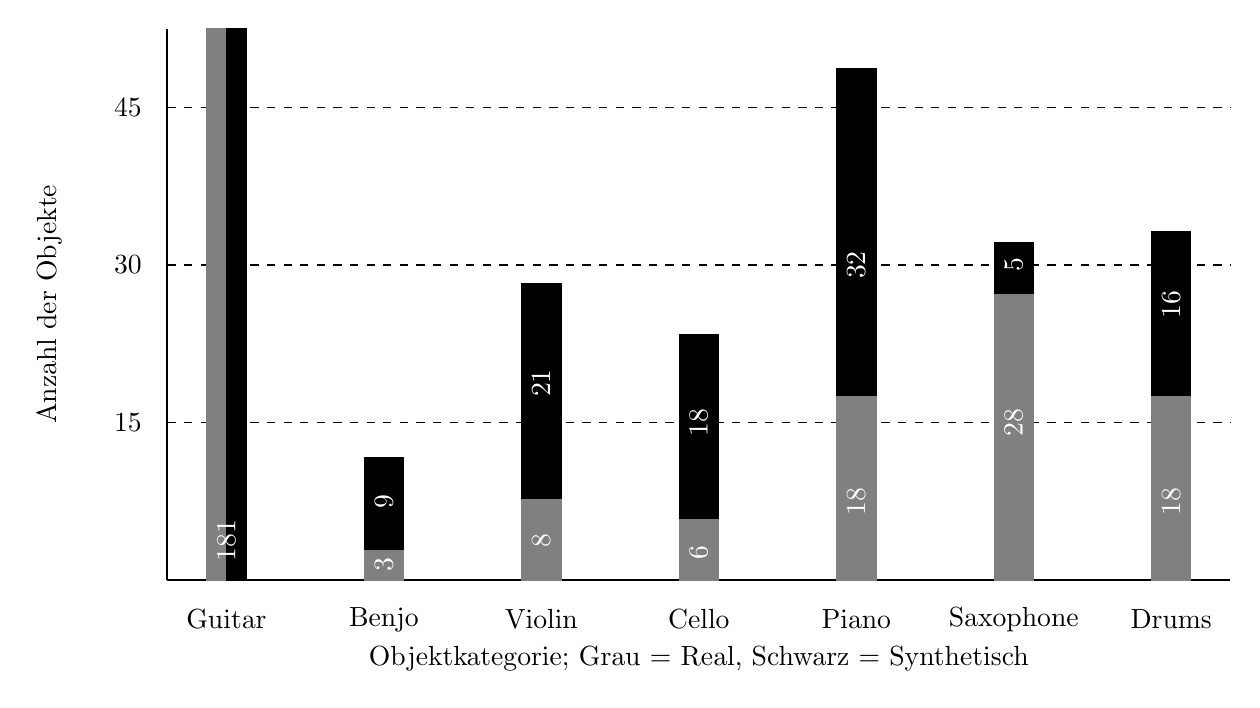
\begin{tikzpicture}
            \draw[thick] (0,0) -- (13.5,0); % x-Achse
            \draw[thick] (0,0) -- (0,7); % y-Achse
            \draw[dashed] (0,2) -- (13.5,2); % y-Achse für die höchste Kategorie
            \draw[dashed] (0,4) -- (13.5,4); % y-Achse für die höchste Kategorie
            \draw[dashed] (0,6) -- (13.5,6); % y-Achse für die höchste Kategorie

            % Real
            \filldraw[gray] (0.5,0) rectangle (0.75,7);
            \filldraw[gray] (2.5,0) rectangle (3,0.39);
            \filldraw[gray] (4.5,0) rectangle (5,1.04);
            \filldraw[gray] (6.5,0) rectangle (7,0.78);
            \filldraw[gray] (8.5,0) rectangle (9,2.34);
            \filldraw[gray] (10.5,0) rectangle (11,3.64);
            \filldraw[gray] (12.5,0) rectangle (13,2.34);

            % Synthetisch
            \filldraw[black] (0.75,0) rectangle (1,7);
            \filldraw[black] (2.5,0.39) rectangle (3,1.56);
            \filldraw[black] (4.5,1.04) rectangle (5,3.77);
            \filldraw[black] (6.5,0.78) rectangle (7,3.12);
            \filldraw[black] (8.5,2.34) rectangle (9,6.5);
            \filldraw[black] (10.5,3.64) rectangle (11,4.29);
            \filldraw[black] (12.5,2.34) rectangle (13,4.42);

            % Beschriftung der Balken Real
            \node[rotate=90, text=white] at (0.75,0.5) {181};
            \node[rotate=90, text=white] at (2.75,0.2) {3};
            \node[rotate=90, text=white] at (4.75,0.5) {8};
            \node[rotate=90, text=white] at (6.75,0.35) {6};
            \node[rotate=90, text=white] at (8.75,1) {18};
            \node[rotate=90, text=white] at (10.75,2) {28};
            \node[rotate=90, text=white] at (12.75,1) {18};

            % Beschriftung der Balken Synthetisch
            % \node[rotate=90, text=white] at (0.75,1) {181};
            \node[rotate=90, text=white] at (2.75,1) {9};
            \node[rotate=90, text=white] at (4.75,2.5) {21};
            \node[rotate=90, text=white] at (6.75,2) {18};
            \node[rotate=90, text=white] at (8.75,4) {32};
            \node[rotate=90, text=white] at (10.75,4) {5};
            \node[rotate=90, text=white] at (12.75,3.5) {16};

            % x-Achsenbeschriftung
            \node at (0.75,-0.5) {Guitar};
            \node at (2.75,-0.5) {Benjo};
            \node at (4.75,-0.5) {Violin};
            \node at (6.75,-0.5) {Cello};
            \node at (8.75,-0.5) {Piano};
            \node at (10.75,-0.5) {Saxophone};
            \node at (12.75,-0.5) {Drums};
            \node at (6.75,-1) {Objektkategorie; Grau = Real, Schwarz = Synthetisch};

            % Y-Achsenbeschriftung
            \node[rotate=90] at (-1.5,3.5) {Anzahl der Objekte};
            \node at (-0.5,2) {15};
            \node at (-0.5,4) {30};
            \node at (-0.5,6) {45};
        \end{tikzpicture}
    }
    \caption{Säulendiagramm zur Auswertung der Anzahl der annotierten Objekte pro Kategorie.}
    \label{fig:annotation_bar_chart}
\end{figure}

Abbildung \ref{fig:annotation_bar_chart} zeigt ein Säulendiagramm der Anzahl der annotierten Objekte pro Kategorie. Dabei ist zu erkennen, dass mit Abstand die meisten Objekte in der Kategorie \emph{Guitar} (Gitarre) annotiert wurden. Da diese weit über den Bereich Wertebereich des Diagramms hinausgehen. Hier enthalten die echten Bilder 81 Instanzen und die generierten Bilder 100 Instanzen. Dies ist sowohl bei den realen als auch bei den synthetischen Bildern mehr als doppelt so viel wie die nächst kleinere Kategorie \emph{Piano} (Klavier). Grundsätzlich ist zu erkennen, dass die Anzahl der Annotationen in den synthetischen Bildern höher ist als in den realen Bildern. Dies kann beim Vergleich der Ergebnisse mit diesen Trainigsdaten zu Verzerrungen führen und sollte bei der weiteren Verwendung beachtet werden. Dies kann zum Beispiel durch das Sammlen von weiteren realen Bildern ausgeglichen werden. Aufgrund der verfügbaren Zeit des Projektes ist dies jedoch in diesem Projekt nicht mehr möglich.

Die JSON-Datei \texttt{real-synth\_image\_annotations.json} im Verzeichnis \texttt{code/dataset} enthält aktuell alle Annotationen für die 100 Bilder. Für ein getrenntes Trainign der realen und generierten Bilder wurden die Annotationen in zwei Dateien aufgeteilt. Die Annotationen der realen Bilder sind in der Datei \texttt{real\_image\_annotations.json} und die Annotationen der synthetischen Bilder in der Datei \texttt{synth\_image\_annotations.json} im jeweiligen Unterverzeichnis der Bilder zu finden.
Dies ermöglicht eine getrennte Verwendung der beiden Teile des Datensatzes, aber auch eine gemeinsame Verwendung, da es innerhalb der JSON-Dateien keine sich überschneidenden IDs gibt.

Um die Verwendbarkeit des Datensatzes zu testen, wurde ein weiteres Jupyter Notebook erstellt, in dem der erstellte Datensatz geladen und für das Training eines Modells verwendet wird.
Um den Datensatz zu laden wird das Modul \texttt{COCODetection} aus dem \texttt{torchvision} Paket verwendet. Dieses Modul ist speziell für das Laden von COCO Datensätzen entwickelt worden und bietet eine einfache Möglichkeit, die Bilder und Annotationen zu laden und zu verarbeiten. 
Um ein \emph{Dataset} Objet zu erstellen, genügt es der Klasse \emph{CocoDetection} den Pfad zu dem Verzeichnis mit den Bildern und den Pfad zur JSON-Datei mit den Annotationen zu übergeben. Zusätzlich wird noch ein Transformationsobjekt übergeben, welches die Bilder in das richtige Format für das Training bringt. In diesem Fall wird das Transformationsobjekt \texttt{ToTensor} verwendet, welches die Bilder in Tensoren umwandelt.
Für das Training wird das \emph{Faster R-CNN} Modell aus dem \texttt{torchvision} Paket verwendet.
Um das Dataset mit diesem Modell nutzen zu können, muss der Datensatz in das richtige Format gebracht werden. Dafür wurde die Funktion \texttt{convert\_target} erstellt. Diese wandelt eine COCO-Annotation in das vom Modell erwartete Format um. Dieses besteht aus einem \emph{Dictionary}, mit den Schlüsseln \texttt{boxes}, \texttt{labels}. Dabei ist \texttt{boxes} eine Liste von \emph{bounding boxes} in der Form \texttt{[x1, y1, x2, y2]}. Die \texttt{labels} sind die IDs der Kategorien, die den Objekten in den Bildern zugeordnet sind. Diese IDs entsprechen den IDs in der JSON-Datei mit den Annotationen.
Die Funktion \texttt{collate\_fn} wird verwendet um die Bilder und Annotationen richtig zuzusammenzuführen.
Anschließend wird wird das Modell mit der \emph{torchvision} Funktion \texttt{train\_fasterrcnn\_resnet50\_fpn} geladen, in den Trainigsmodus versetzt und, falls möglich, auf eine GPU verschoben. Das Modell wird dann in 10 Epochen und einem \emph{SGD-Optimizer} trainiert.
Als Ergebnis wird in der ersten Epoche ein Loss von 25.9 erreicht und in der zehnten Epoche ein Loss von 4.6.

\section{Projektabschluss}
Mit dem Erfolg des Tests des Datensatzes wurde das Projekt erfolgreich und innerhalb der Zeitvorgaben abgeschlossen. 
Zusammenfassend wurden im Rahmen dieses Projekts sowohl echte als auch synthetische Bilder gesammelt, sorgfältig annotiert und in einem einheitlichen Format bereitgestellt. Durch die Evaluation verschiedener Bildgenerierungsmodelle konnte ein geeignetes Modell für die Erstellung synthetischer Daten ausgewählt werden. Die Annotation im COCO-Format ermöglicht eine direkte Weiterverwendung mit etablierten Frameworks und Modellen im Bereich der Objekterkennung.
Die im Projekt gewonnenen Erkenntnisse und der erstellte Datensatz bilden eine solide Grundlage für weiterführende Arbeiten, insbesondere für die geplante Bachelorarbeit, in der die Leistungsfähigkeit von Objekterkennungsmodellen auf Basis dieses Datensatzes untersucht werden soll. Darüber hinaus kann der Workflow zur Datensatzgenerierung und -annotation als Vorlage für ähnliche Projekte dienen.
Die Ergebnisse des Projektes werden in einer noch folgenden abschließenden Präsentation vorgestellt.

Die vollständigen Dateien des Projekts, einschließlich der generierten Bilder, Annotationen und Jupyter Notebooks, sind im GitHub Repository \url{https://github.com/fhswf-projekte/real-synth-object-detection-dataset-titom001} verfügbar.
